\documentclass[a0,portrait]{a0poster}


\usepackage{multicol}
\columnsep=100pt
\columnseprule=3pt


\usepackage{times}
\usepackage{graphicx}
\graphicspath{{../}}
\usepackage{booktabs}
\usepackage[font=small,labelfont=bf]{caption}
\usepackage{amsfonts, amsmath, amsthm, amssymb, marvosym}
\usepackage{wrapfig}
\usepackage{enumitem}
\usepackage{fancyvrb}
\usepackage{xspace}
\usepackage[svgnames,usenames,dvipsnames]{xcolor}
\usepackage[utf8]{inputenc}


%\usepackage{algorithm}
%\usepackage[noend]{algorithmic}
\usepackage{algpseudocode}


\def\texttts#1{\texttt{\large#1}}


\begin{document}
	
	
%---------------------------------------------------------------
%	POSTER HEADER 
%---------------------------------------------------------------
\begin{minipage}[t]{0.15\linewidth}
	\vspace{-13cm}
	\hspace*{2cm}
	
\includegraphics[width=8cm]{fig/logoPUCRS.pdf}
\end{minipage}
\begin{minipage}[b]{0.65\linewidth}
	\begin{center}
	\veryHuge \color{NavyBlue} 
	\textbf{Adversarial Hierarchical-Task Network \\para Jogos em Tempo Real} 
	\color{Black}\\%[1cm] % Subtitle
	\huge \textbf{Matheus de Souza Redecker} \\
	\Large \textbf{Orientador: Prof. Felipe Rech Meneguzzi}\\
	\Large Pontifícia Universidade Católica do Rio Grande do Sul (PUCRS) -- Faculdade de Informática (FACIN)\\ 
	Curso de Ciência da Computação \\
	%Porto Alegre -- RS -- Brasil\\ % University/organization
	\Large \Letter ~ \texttt{matheus.redecker@acad.pucrs.br}%\\
	%\Large \Letter ~ \texttt{felipe.meneguzzi@pucrs.br}
	\end{center}
\end{minipage}
\hspace*{1cm}
\begin{minipage}[t]{0.15\linewidth}
	\vspace{-12cm}
	\hspace*{2cm}
	
\includegraphics[width=8cm]{fig/logoFacin.pdf}
\end{minipage}
\vspace{2cm}

%---------------------------------------------------------------

\begin{multicols}{2} 
%---------------------------------------------------------------
%	ABSTRACT
%---------------------------------------------------------------
	\color{NavyBlue}
	\color{Black}
	\raggedright
	\Large
	\newcommand\itemadjust{\itemsep.5em \parskip0pt \parsep0pt}
%---------------------------------------------------------------
%	Motivação
%---------------------------------------------------------------
	\color{NavyBlue}
	\section*{\huge Motiva\c{c}\~ao}
	\color{Black}
	
	\begin{itemize}
		%[leftmargin=2em]\itemadjust
		\item Nos jogos de computador as reações das jogadas devem ser quase que imediatas, por esse motivo técnicas que tentam explorar todas as possibilidades possíveis de um jogo se tornam inviáveis para jogos com uma complexidade alta.
		\item Por exemplo, no xadrez a quantidade aproximada de estados possíveis é de $10^{40}$, isso mostra que é preciso algoritmos eficientes para gerar uma ação de maneira rápida. 
		\item O intuito deste trabalho é explorar eficientemente o espaço de ações disponíveis usando conhecimento de domínio, a fim de definir qual a próxima ação que deve ser executada. Para isso, propomos a utilização do algoritmo de Adversarial Hierarchical-Task Network (AHTN).
		\item Para rodar os experimentos escolhemos a plataforma MicroRTS, que é um jogo de estratégia em tempo real. 
	\end{itemize}

%---------------------------------------------------------------
%   Background
%---------------------------------------------------------------
	\color{NavyBlue}
	\section*{\huge Background}
	\color{Black}
		
	\textbf{Adversarial Hierarchical-Task Network}
		\begin{itemize}
			%[leftmargin=2em]\itemadjust
			\item O AHTN é um algoritmo desenvolvido para lidar com o problema do grande fator de ramificação dos jogos em tempo real.
			\item Ele utiliza conhecimento de domínio no estilo de planejamento hierárquico (HTN).
			\item No algoritmo são combinados técnicas de HTN com o algoritmo \textit{minimax search}.
			\item O algoritmo assume jogos totalmente observáveis, baseados em turno e determinísticos. 
		\end{itemize}
		
		\vspace{8mm}
		
		{\large
		\begin{algorithmic}[1]
			\Function {AHTNMax}{$s, N_{+}, N_{-}, t_{+}, t_{-}, d$}
			\If {$terminal(s) \vee d \leq 0$}\label{alg:lin:firstLine}
			\State	\Return $(N_{+}, N_{-}, e(s))$
			\EndIf
			\If {$nextAction(N_{+}, t_{+}) \neq \perp$} \label{alg:ahtn:nexaction}
			\State $t = nextAction(N_{+}, t_{+})$ 
			\State \Return $\Call{AHTNMin}{(\gamma(s,t), N_{+}, N_{-}, t, t_{-}, d-1)}$ \label{alg:ahtn:troca}
			\EndIf
			\State $N_{+}^{*} = \perp, N_{-}^{*} = \perp, v^{*} = -\infty$
			\State $\aleph = decompositions_{+}(s, N_{+}, N_{-}, t_{+}, t_{-})$ \label{alg:decompositions}
			\ForAll{$N \in \aleph$} \label{alg:ahtn:for}
			\State $(N^{'}_{+}, N^{'}_{-}, v^{'}) = AHTNMax(s, N, N_{-}, t_{+}, t_{-}, d)$
			\If{$v^{'} > v^{*}$}
			\State $N_{+}^{*} = N^{'}_{+}, N_{-}^{*} = N^{'}_{-}, v^{*} = v^{'} $
			\EndIf
			\EndFor		
			\State \Return $(N_{+}^{*}, N_{-}^{*}, v^{*} )$
			\EndFunction
		\end{algorithmic}
	}
		\vspace{10mm}
		
	\textbf{Simple Hierarchical Ordered Planner 2}
		\begin{itemize}
			%[leftmargin=2em]\itemadjust
			\item Simple Hierarchical Ordered Planner 2 (SHOP2) é um sistema de planejamento independente de domínio baseado em planejamento hierárquico (HTN).
			\item O SHOP2 precisa de uma descrição do domínio e uma descrição do problema para gerar os planos.
			\item A descrição do domínio é a descrição do domínio de planejamento, onde estão descritos os métodos e operadores.
			\item Já a descrição do problema, é onde está descrito o estado inicial as tarefas que desejam ser alcançadas.
		\end{itemize}
		
		\vspace{10mm}
	\textbf{MicroRTS}
		\begin{itemize}
			[leftmargin=2em]\itemadjust
			\item O MicroRTS é um jogo de estratégia em tempo real (RTS).
			\item Ele é uma simplificação do jogo Starcraft, feito por Santiago Ontañón.
			\item O MicroRTS foi desenvolvido para fins acadêmicos, com o intuito de aplicar e desenvolver técnicas de Inteligência Artificial.
		\end{itemize}
		
		\vspace{8mm}
		
		\begin{center}
			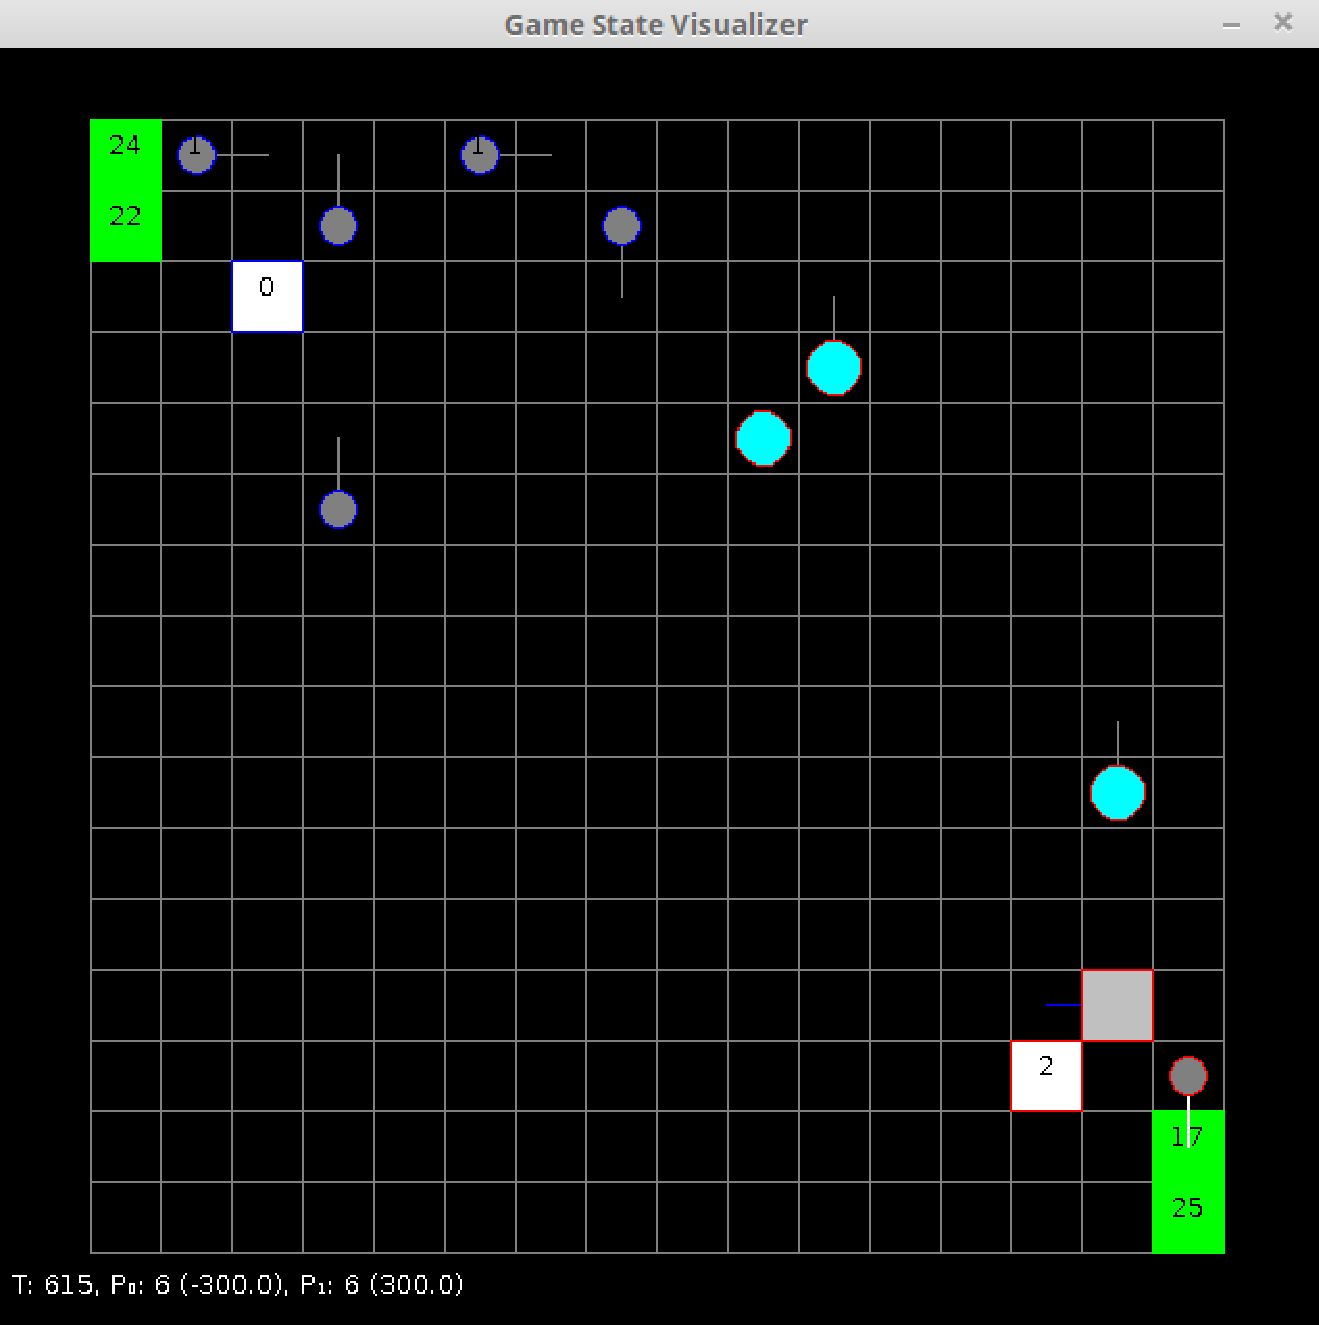
\includegraphics[width=0.5\linewidth]{fig/microRts.pdf}
			\captionof{figure}{Exemplo de tela de um jogo do MicroRTS.}
		\end{center}	
		
%---------------------------------------------------------------
%	Implementação
%---------------------------------------------------------------
	\color{NavyBlue}
	\section*{\huge Implementação}
	\color{Black}
	\begin{itemize}
		%[leftmargin=2em]\itemadjust
		\item A implementação do algoritmo foi feita na plataforma do MicroRTS, utilizando o SHOP2 para geração dos planos.
		\item Foram criados dois conhecimento de domínio pensando em um cenário de jogo onde o jogador cria tropas para mandar destruir a base adversária.
		\item A primeira estratégia cria apenas uma unidade de ataque por vez e em seguida manda atacar. Já a segunda estratégia enquanto está atacando também cria novas tropas.  
	\end{itemize}

%---------------------------------------------------------------
%	Experimentos e Resultados
%---------------------------------------------------------------
	\color{NavyBlue}
	\section*{\huge Experimentos e resultados}
	\color{Black}

	\begin{itemize}
		%[leftmargin=2em]\itemadjust
		\item Os experimentos a seguir foram executados em um mapa 16 por 16, com cada jogador inicialmente possuindo uma base, um trabalhador e dois recursos próximos a sua base. 
		\cite{nau2003shop2}\cite{ontanon2013combinatorial}\cite{ontanon2015adversarial}
		\item O MicroRTS possui algumas técnicas de jogo implementadas, que podem ser jogados contra.
		\item O algoritmo de AHTN foi testado contra algumas dessas técnicas começando dos dois lados do jogo, azul na parte superior, e vermelho na parte inferior.
	\end{itemize}
	
	\vspace{8mm}
	{\large
	\begin{center}
		\begin{tabular}{|c|cc|cc|}
			\hline
			\textbf{}           & \multicolumn{2}{c|}{\textbf{Lado Azul}}                    & \multicolumn{2}{c|}{\textbf{Lado Vermelho}}                \\ \hline
				\textbf{Adversário} & \multicolumn{1}{c|}{\textbf{Vitórias}} & \textbf{Derrotas} & \multicolumn{1}{c|}{\textbf{Vitórias}} & \textbf{Derrotas} \\ \hline
				\multicolumn{5}{|c|}{\textbf{Estrat\'egia 1}}                                                                                                   \\ \hline
				RandomAI              & 5                                      & 0                 & 5                                      & 0                 \\
				RangedRush              & 0                                      & 5                 & 5                                      & 0                 \\
				HeavyRush               & 0                                      & 5                 & 5                                      & 0                 \\
				LightRush               & 0                                      & 5                 & 5                                      & 0                 \\
				WorkerRush              & 0                                      & 5                 & 0                                      & 5                 \\ \hline
				\multicolumn{5}{|c|}{\textbf{Estrategia 2}}                                                                                                   \\ \hline
				RandomAI              & 5                                      & 0                 & 5                                      & 0                 \\
				RangedRush              & 5                                      & 0                 & 5                                      & 0                 \\
				HeavyRush               & 0                                      & 5                 & 5                                      & 0                 \\
				LightRush               & 0                                      & 5                 & 5                                      & 0                 \\
				WorkerRush              & 0                                      & 5                 & 0                                      & 5                 \\ \hline
		\end{tabular}
		\captionof{table}{Resultado do algoritmo contra técnicas do MicroRTS.}
	\end{center}
	}

%---------------------------------------------------------------
%	Referencias
%---------------------------------------------------------------
	%\large
	%\color{NavyBlue}
	%\section*{Referências}
	%\renewcommand{\section}[2]{}
	%\color{Black}
	%\raggedright
	%\bibliographystyle{plain}
	%\bibliography{poster}
			
\end{multicols}
\end{document}


